\documentclass[tikz, border=6pt]{standalone}
\usepackage[T1]{fontenc}
\usepackage{lmodern}
\usepackage{amsmath,amssymb,bm}
\usepackage{lmodern}
\usetikzlibrary{arrows.meta, calc, fit, backgrounds, matrix}
\definecolor{Blue}{HTML}{3A76D8}
\definecolor{Green}{HTML}{3BA55C}
\definecolor{Orange}{HTML}{EE8133}
\definecolor{Ink}{HTML}{1F2937}
\begin{document}
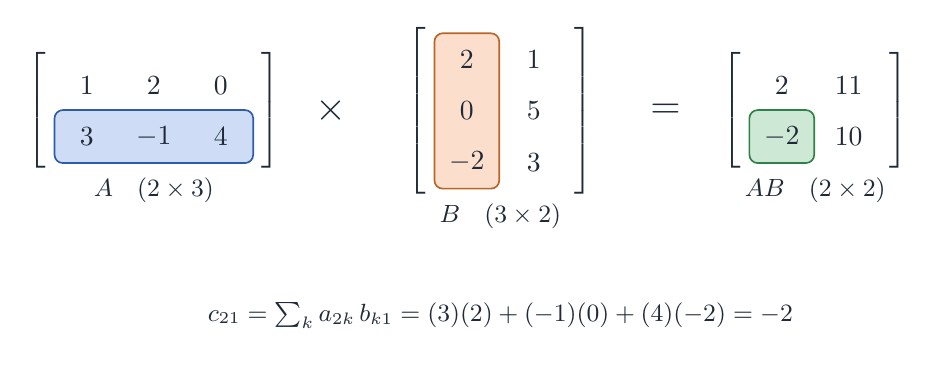
\begin{tikzpicture}[color=Ink, line width=0.5pt, >={Latex[length=5pt, width=3.6pt]}, line join=round]
  \matrix[matrix of math nodes, anchor=center, left delimiter={[}, right delimiter={]}, column sep=0.15cm, row sep=0.1cm, nodes={minimum width=0.7cm, minimum height=0.55cm, anchor=center, inner sep=1pt}] (A) at (0,0) {
    1 & 2 & 0 \\
    3 & -1 & 4 \\
  };
  \begin{scope}[on background layer]
    \node[fit=(A-2-1)(A-2-3), inner sep=1.5pt, rounded corners=3pt, fill=Blue!25, draw=Blue!78!black, line width=0.6pt] {};
  \end{scope}
  \node[anchor=north, font=\small] at (A.south) {$A$ \; ($2\times 3$)};
  \matrix[matrix of math nodes, anchor=center, left delimiter={[}, right delimiter={]}, column sep=0.15cm, row sep=0.1cm, nodes={minimum width=0.7cm, minimum height=0.55cm, anchor=center, inner sep=1pt}] (B) at (4.4,0) {
    2 & 1 \\
    0 & 5 \\
    -2 & 3 \\
  };
  \begin{scope}[on background layer]
    \node[fit=(B-1-1)(B-3-1), inner sep=1.5pt, rounded corners=3pt, fill=Orange!25, draw=Orange!78!black, line width=0.6pt] {};
  \end{scope}
  \node[anchor=north, font=\small] at (B.south) {$B$ \; ($3\times 2$)};
  \matrix[matrix of math nodes, anchor=center, left delimiter={[}, right delimiter={]}, column sep=0.15cm, row sep=0.1cm, nodes={minimum width=0.7cm, minimum height=0.55cm, anchor=center, inner sep=1pt}] (C) at (8.4,0) {
    2 & 11 \\
    -2 & 10 \\
  };
  \begin{scope}[on background layer]
    \node[fit=(C-2-1), inner sep=1.5pt, rounded corners=3pt, fill=Green!25, draw=Green!78!black, line width=0.6pt] {};
  \end{scope}
  \node[anchor=north, font=\small] at (C.south) {$AB$ \; ($2\times 2$)};
  \node[font=\Large] at (2.25,0) {$\times$};
  \node[font=\Large] at (6.5,0) {$=$};
  \node[font=\small] at (4.4,-2.6) {$c_{21} = \sum_k a_{2k}\, b_{k1} = (3)(2) + (-1)(0) + (4)(-2) = -2$};
\end{tikzpicture}
\end{document}
